\documentclass[a4paper]{scrartcl}
\usepackage{amsmath}
\usepackage{tikz}
\usetikzlibrary{patterns}

\begin{document}

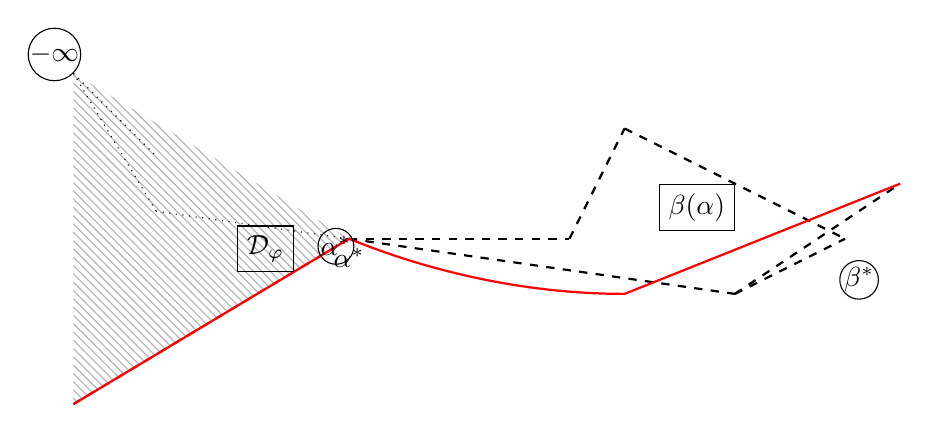
\begin{tikzpicture}[scale=.7]
% draw the curve and label it
\draw[thick,red,dashed] (-6,-3)--(-1,0);
\node[below] at (-1,0){$\alpha^\ast$};
\draw[thick,dashed] (3,0)--(4,2);
\draw[thick,dashed] (6,-1)--(9,1);
\draw[thick,dashed] (-1,0)--(3,0);
\draw[thick,dashed] (-1,0)--(6,-1);
\draw[thick,dashed] (4,2)--(8,0);
\draw[thick,dashed] (6,-1)--(8,0);
% fill area and draw dotted lines
\fill[pattern=north west lines,pattern color=black!30] (-6,-3)--(-6,3)--(-1,0)--cycle;
\draw[dotted] (-6,3)--(-4.5,1.5);
\draw[dotted] (-6,3)--(-4.5,.5);
\draw[dotted] (-4.5,.5)--(-1,0);
% draw the curve and label it
\draw[thick,red] (-6,-3)--(-1,0) parabola[bend at end,bend angle=130](4,-1)--(9,1);
\node[rectangle,draw,anchor=south east] at (-2, -.6){$\mathcal{D}_{\varphi}$};
\node[rectangle,draw,anchor=north east] at (6, 1){$\beta(\alpha)$};
\node[circle,inner sep=0pt,minimum size=.1cm,draw,anchor=south west] at (8, -1){$\beta^\ast$};
\node[circle,inner sep=0pt,minimum size=.1cm,draw,anchor=north east] at (-1, .1){$\alpha^\ast$};
\node[circle,inner sep=0pt,minimum size=.1cm,draw,anchor=south east] at (-6, 3){$-\infty$};
\end{tikzpicture}

\end{document}